%%%%%%%%%%%%%%%%%%%%%%%%%%%%%%%%%%%%%%%%%%%%%%%%%%%%%%%%%%%%
%         file: report.tex
%         date: 26 feb 2017
%       author: S <scassiau@enseirb-matmeca.fr>
%  description: CS551 Project 1 report
%%%%%%%%%%%%%%%%%%%%%%%%%%%%%%%%%%%%%%%%%%%%%%%%%%%%%%%%%%%%

\documentclass[fleqn]{article}

%\usepackage[francais]{babel}
\usepackage[utf8]{inputenc}
\usepackage[T1]{fontenc}
\usepackage[letterpaper,scale=0.80]{geometry}
\usepackage{amsmath}
\usepackage{amssymb}
\usepackage{stmaryrd}
\usepackage{fancyhdr}
%\usepackage{graphicx}
\usepackage{tikz}
\usetikzlibrary{arrows,automata,positioning}
\usepackage{multicol}
\usepackage{listings}
\usepackage{color}
\usepackage{textcomp}
\usepackage{framed}

\newcommand{\bull}{•}

\pagestyle{fancy}
\lfoot{CS551 - Project 1 - Develop your own shell}
\rfoot{Benoît Lafon - Sylvain Cassiau}

\renewcommand{\headrulewidth}{0pt}
\renewcommand{\footrulewidth}{0.4pt}

\title{CS551 OS Design and Implementation\\Project 1 - Develop your own shell}
\author{Benoît Lafon - Sylvain Cassiau}
\date{February 27, 2017}

\begin{document}

\maketitle

\begin{center}
\line(1,0){150}
\vspace{1cm}
\end{center}


\begin{figure}
    \centering
    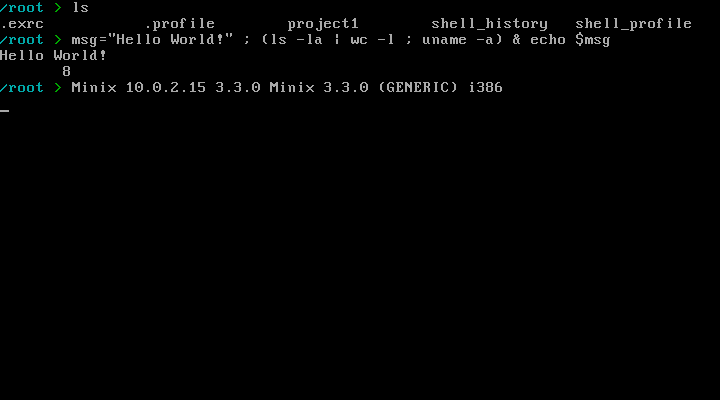
\includegraphics[width=\textwidth]{screenshot}
    \caption{Screenshot of our shell}
    \label{fig:screenshot}
\end{figure}


\section{Parsing}

In order to parse commands from either a script or a prompt in an efficient and robust way, we decided to use the GNU tools \texttt{Lex} and \texttt{Yacc}.
\texttt{Lex} splits a command into tokens and \texttt{Yacc} builds a structured representation of this command using the Object-Oriented pattern described in section \ref{sec:oop}.
To do so, we first had to define the grammar that rules the semantic and syntax of the commands to parse. These tokens and rules can be respectively found in \texttt{scanner.l} and \texttt{grammar.y} files.

Here is a quick summary of the supported syntax:
\begin{itemize}
    \item commands with zero, one, or multiple arguments. e.g. \texttt{ls -l /usr/bin}. If a command or argument contains spaces, quotes can be used to delimit its beginning and end. e.g. \texttt{cmd "argument with spaces" "support escaped characters like \textbackslash""}
    \item sequences of commands separated by \texttt{;} or \texttt{\&}. The \texttt{;} symbol means that the preceding command is run in foreground, whereas \texttt{\&} means that the preceding command is run in background. An implicit \texttt{;} is added at the end of the command line if no separator is specified. e.g. \texttt{cmd1 ; cmd2 \& cmd3}
    \item as a bonus functionality, the standard output of a command can be piped to the standard input of an other command with the symbol \texttt{|}. e.g. \texttt{cmd1 | cmd2 | cmd3}
    \item commands can be grouped between \texttt{(} and \texttt{)} to be executed as a block. e.g. in the command line \texttt{(cmd1 ; cmd2) \& cmd3}, the whole group \texttt{cmd1 ; cmd2} is executed in background while \texttt{cmd3} is executed in foreground.
    \item variables can be defined like this: \texttt{var=content}. And their content is accessed like this: \texttt{\$var}. The variable replacement process is applied to all commands and arguments before they are executed.
\end{itemize}

\section{Object-Oriented Design}
\label{sec:oop}

For a better code understanding and an easier maintenance, we chose to follow an Object-Oriented pattern. Of course, \texttt{C} is not a language designed for Object-Oriented Programming. Therefore, we do not really have classes and objects. Instead, we used structures to represent the formal objects that we had to manipulate, and functions to manipulate these structures. For example, the structure \texttt{command} is used by \texttt{command\_\_new()}, \texttt{command\_\_append\_arg()}, \texttt{command\_\_execute()} or \texttt{command\_\_free()}. Therefore, it becomes much clearer to distinguish which methods belong to which structures.


\section{Input}

The default way user input is managed in a terminal is called canonical mode. This means that the operating system is buffering the input, so that the user can move the input cursor, erase or edit. The buffer is sent to the program once the user presses the return key and can be accessed by one or multiple calls to the read function. This canonical mode does not permit to read which key has been pressed before the user presses return. Therefore, it is not possible to detect a [TAB] press for the auto-completion. In order to read keys directly, we decided to turn off the canonical mode. By doing so, we can capture each keyboard event individually and assign a different action for each of them. Those include re-implementing the action of the left and right arrows keys to move the cursor, erasing a character with the backspace key, inserting a new character and so on. Moreover, this low level of operation allows us to implement the auto-completion functionality as described in section \ref{sec:auto}. Only when the user exits the shell, the canonical mode is switched back on making the transition between two shell executions transparent.



\section{Auto-completion}
\label{sec:auto}

Auto-completion has been implemented using a double linked list. Each time the user executes a non empty command, the latter is pushed into the list.
The list has a maximum size, therefore if the size is exceeded when pushing a new element, the last one is automatically popped.
When the user ends the execution of the shell, the list of commands is saved into a file. If the file already exists, then it will be overwritten, otherwise a new file is created.
This same file will also be read each time the user runs the shell allowing to load back all their previous command history.
The user can browse this history backward by using [TAB] or [ARROW UP] keys. Conversely, [ARROW DOWN] will browse forward.
If the cursor is at the left-most position, then all the history will be considered.
However, if the user starts typing or place the cursor at a given position other than the left-most one, then the auto-completion will consider commands that match all characters from the beginning of the prompt until the current cursor position.
If the user is not satisfied about the auto-completion suggestions, they can always come back to their original typing command by arrowing down repetitively to the most recent history command that matches their typing command.

\section{Exception Handling}

We used the return value to check if the execution of a system call went well. If not, our shell prints a descriptive message on the standard error output describing the reason of the error. Most of the time it is not possible to easily recover from the error and we chose to exit the shell after the error message display.

All memory allocations (\texttt{malloc}, \texttt{realloc}, \texttt{strdup}) are wrapped into custom functions checking if the allocation was performed correctly. If not, the shell writes the issue on the standard error output and exit.

In some error situations, it is possible to recover. For example if a file (profile or command history) is missing, the shell uses default empty values.

\section{Shell Environment}

In order to fully exploit the shell, a profile file is read when initializing the shell. The file is mainly used to set the environment variables such that \texttt{\$PATH} and \texttt{\$HOME}. By doing so, the shell will have access to the set of executable programs available in the specified directories.
However, even if the \texttt{\$PATH} variable is not set, it is considered empty, and the user can still have access to the built-in functions of the shell, or execute programs by specifying their absolute path. Two built-ins are actually implemented. They are the most fundamental ones: the first one is \texttt{cd()}; allowing to change directory in MINIX. The other built-in is \texttt{exit()} for quitting the shell alongside with \texttt{Ctrl-D}. Both trigger the same action.

To improve the shell experience for the user, the current working directory is included in each displayed prompt.

A special functionality of the shell is the alarm that can be turned off or on from the profile file via the \texttt{\$ALARM} variable. If set on, an informative message will be printed on the screen as soon as the user executes a command whose duration exceeds 5 seconds informing the users that they can kill the processes including the children by pressing \texttt{Ctrl-C}.
The alarm is triggered via a signal \texttt{SIGALRM}. It is not blocking and does not grant the user special rights over the running program. Therefore, the user can kill a program at any time even though the alarm is set off.

\section{Tests}

We wrote automated functional tests for our shell.
Test cases are scripts covering all functionalities of the shell. They were written to test progressively more and more complex commands with both authorized commands or command errors. Each script is covering a specific domain.
The testing process consists in executing these scripts.
The standard and error outputs of each executed script are saved into files and are then compared to files containing the expected standard and error outputs.
If each pairwise comparison matched syntactically, the test is considered to be valid.
If the comparison does not match, the difference between the expected output and the produced one is printed with the \texttt{diff} program.

\end{document}
